\documentclass{beamer}

\usepackage{graphicx}
\usepackage{listings}
\usepackage{hyperref}

\lstset{
  basicstyle=\scriptsize,
  columns=fixed,
  frame=none,
  backgroundcolor=\color[RGB]{245,245,244},
  keywordstyle=\color[RGB]{40,40,255},
  numberstyle=\scriptsize\color{darkgray},
  comment=[l]{--},
  commentstyle=\it\color[RGB]{0,96,96},
  stringstyle=\rmfamily\slshape\color[RGB]{128,0,0},
  showstringspaces=false,
  morekeywords={terra, if, else, end, int, then, return, struct, float, local, quote, function, var, for, do}
}

\usetheme{AnnArbor}
\usecolortheme{beaver}

\begin{document}
\title{Terra: A Multi-Stage Language for High-Performance Computing}
\author{Presenter: Cunyuan}

\maketitle

\def\LArr{\xrightarrow[]{L}}
\def\SArr{\xrightarrow[]{S}}
\def\TArr{\xrightarrow[]{T}}
\def\ude#1{\underline{\dot{#1}}}

\begin{frame}
	\frametitle{Goals}
  \begin{itemize}
  \item Performance matters!\pause
  \item Low-level languages(e.g. C) are good: we need to make best use of features of the target architecture(e.g. vector instructions).\pause
  \item Programming is difficult!\pause
  \item Solution: use high-level languages to generate low-level languages code(e.g. FFTW: OCaml $\rightarrow$ C).
  \end{itemize}
\end{frame}

\begin{frame}
	\frametitle{New Problems}
  \begin{itemize}
  \item In this case, we get three components.\pause
  \item Optimizer: generate plan to guide how to generate code.\pause
  \item Compiler: generate target code based on the plan.\pause
  \item Runtime: support the generated code and provide feedback to the optimizer.\pause
  \item Problem1: Separating compiler and optimizer from the runtime makes it difficult to feed runtime statistics back to the compiler to perform problem-specific optimizations.\pause
  \item Problem2: How can we re-use legacy libraries?
  \end{itemize}
\end{frame}

\begin{frame}
  \frametitle{Two-Language Design}
  \begin{itemize}
  \item Lua: high-level, dynamically typed, automatic mm, first class functions.\pause
  \item Terra(new!): statically typed, manumal mm.\pause
  \item Use Lua to manipulate Terra code.\pause
  \item Shared lexical scoping, which is hygienic.\pause
  \item Terra code runs independently, to avoid including high-level features.\pause
  \item Lua's stack-based C API makes it easy to interface with legacy code.
  \end{itemize}
\end{frame}

\begin{frame}
	\frametitle{Two-Language Design}
  \begin{center}
    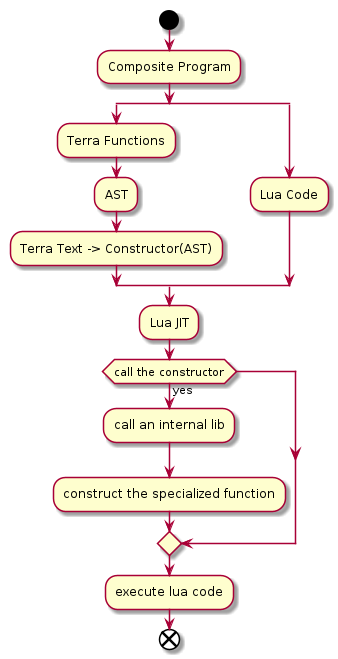
\includegraphics[scale=0.3]{terra.png}
  \end{center}
\end{frame}

\begin{frame}[fragile]
	\frametitle{Some Code Examples}
  \begin{lstlisting}
    terra min(a: int, b: int): int
      if a < b then return a
      else return b end
    end
    struct GreyScaleImage {
      data: &float
      N: int
    }
  \end{lstlisting}
\end{frame}

\begin{frame}
	\frametitle{Features}
  \begin{itemize}
  \item Terra entities are all first-class Lua values.\pause
  \item Terra functions will be executed in LLVM JIT.\pause
  \item You can dump Terra functions to an object file(i.e. something.o in Linux) if you like.\pause
  \item Quotation: using brackets($[]$) for escaping and backtick(expressions)/quote keyword(statements) for creating quotation.
  \end{itemize}
\end{frame}

\begin{frame}[fragile]
  \frametitle{Quotation Example}
  \begin{lstlisting}
    local a = 5
    terra sin5()
      return [ math.sin(a) ]
      end
    function addtwo(a,b)
      return `a + b
    end
    local printtwice = quote
      C.printf("hello\n")
      C.printf("hello\n")
    end
  \end{lstlisting}
\end{frame}

\begin{frame}
	\frametitle{It Just Works!}
  \begin{center}
    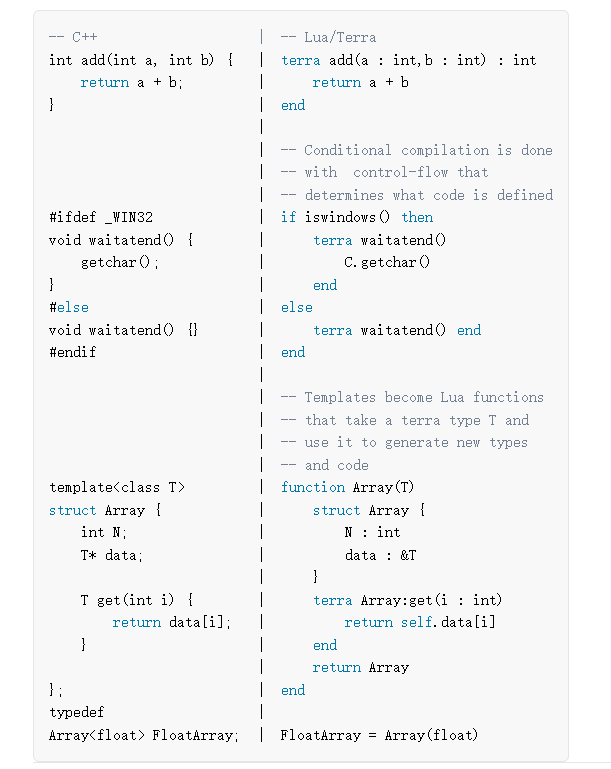
\includegraphics[scale=0.45]{terra2.png}
  \end{center}
\end{frame}

\begin{frame}
	\frametitle{It Just Works!}
  \begin{itemize}
  \item Now we can generate code dynamically.\pause
  \item e.g. block the loop nests to make the memory access more friendly to the cache.
  \end{itemize}
\end{frame}

\begin{frame}[fragile]
  \frametitle{A Simple Filter Example}
  \begin{lstlisting}
GreyscaleImage = Image(float)
terra laplace(img: &GreyscaleImage,
out: &GreyscaleImage) : {}
  --shrink result, do not calculate boundaries
  var newN = img.N - 2
  out:init(newN)
  for i = 0,newN do
    for j = 0,newN do
      var v = -img:get(i+0,j+1) - img:get(i+2,j+1)
      - img:get(i+1,j+2) - img:get(i+1,j+0)
      + 4 * img:get(i+1,j+1)
      out:set(i,j,v)
    end
  end
end
  \end{lstlisting}
\end{frame}

\begin{frame}[fragile]
	\frametitle{A Simple Filter Example}
  \begin{lstlisting}
terra runlaplace(input: rawstring,
output: rawstring) : {}
  var i = GreyscaleImage {}
  var o = GreyscaleImage {}
  i:load(input)
  laplace(&i,&o)
  o:save(output)
  i:free(); o:free()
end
  \end{lstlisting}
\end{frame}

\begin{frame}[fragile]
	\frametitle{Optimize The Filter}
  \begin{lstlisting}
function blockedloop(N,blocksizes,bodyfn)
  local function generatelevel(n,ii,jj,bb)
    if n > #blocksizes then
      return bodyfn(ii,jj)
    end
    local blocksize = blocksizes[n]
    return quote
      for i = ii,min(ii+bb,N),blocksize do
        for j = jj,min(jj+bb,N),blocksize do
          [ generatelevel(n+1,i,j,blocksize) ]
        end
      end
    end
  end
  return generatelevel(1,0,0,N)
end
  \end{lstlisting}
\end{frame}

\begin{frame}[fragile]
	\frametitle{Optimize The Filter}
  \begin{lstlisting}
GreyscaleImage = Image(float)
terra laplace(img: &GreyscaleImage,
out: &GreyscaleImage) : {}
  --shrink result, do not calculate boundaries
  var newN = img.N - 2
  out:init(newN)
  [blockedloop(newN,{128,64,1}, function(i,j)
    return quote
      var v = -img:get(i+0,j+1) - img:get(i+2,j+1)
      - img:get(i+1,j+2) - img:get(i+1,j+0)
      + 4 * img:get(i+1,j+1)
      out:set(i,j,v)
    end
  end)]
end
  \end{lstlisting}
\end{frame}

\begin{frame}
	\frametitle{The Formal Calculus: Terra Core}
  \begin{itemize}
  \item For simplicity, Lua := imperative language + first-class functions, Terra := purely functional language\pause
  \item Lua expression: $e$, evaluation of Lua: $\LArr$\pause
  \item Terra expression: $\dot{e}$, specialization of Terra: $\SArr$\pause
  \item Specialized Terra expression: $\ude{e}$, execution of specailized Terra expression: $\TArr$
  \end{itemize}
\end{frame}

\begin{frame}
	\frametitle{Terra Core}
  Lua Syntax:
  \newline
  \begin{equation}
    \begin{split}
      e\thickspace ::=\thickspace & b\thickspace |\thickspace \dot{T}\thickspace |\thickspace x\thickspace |\thickspace let\thickspace x\thickspace =\thickspace e\thickspace in\thickspace e\thickspace |\thickspace x\thickspace :=\thickspace e\thickspace |\thickspace e(e)\thickspace |\thickspace fun(x)\{e\}\thickspace |\thickspace tdecl\thickspace | \\ & ter\thickspace e(x:\thickspace e):\thickspace e \{\dot{e}\}\thickspace |\thickspace \backprime \dot{e}\\
      v\thickspace ::=\thickspace & b\thickspace |\thickspace l\thickspace |\thickspace \dot{T}\thickspace |\thickspace <\Gamma, x, e>\thickspace |\thickspace \ude{e}\\
      \dot{T} ::=\thickspace & \dot{B}\thickspace |\thickspace \dot{T} \rightarrow \dot{T}
    \end{split} \notag
  \end{equation}
\end{frame}

\begin{frame}
	\frametitle{Terra Core}
  Terra Syntax:
  \newline
  \begin{equation}
    \begin{split}
      \dot{e}\thickspace ::=\thickspace & b\thickspace |\thickspace x\thickspace | \dot{e}(\dot{e}) |\thickspace tlet\thickspace x:\thickspace e\thickspace =\thickspace \dot{e}\thickspace in\thickspace \dot{e}\thickspace |\thickspace [e]\\
      \ude{e}\thickspace ::=\thickspace & b\thickspace |\thickspace\ude{x}\thickspace | \ude{e}(\ude{e}) |\thickspace tlet\thickspace \ude{x}:\thickspace \dot{T}\thickspace =\thickspace \ude{e}\thickspace in\thickspace \ude{e}\thickspace |\thickspace l
    \end{split} \notag
  \end{equation}
\end{frame}

\begin{frame}
  \frametitle{Terra Core}
  \begin{equation}
    v\thickspace \Sigma \LArr v\thickspace \Sigma \tag{LVAL}
  \end{equation}
  \newline
  \begin{equation}
    \frac{\Sigma = \Gamma, S, F}{x\thickspace \Sigma \LArr S(\Gamma{(x)})\thickspace \Sigma}\tag{LVAR}
  \end{equation}
  \newline
  \begin{equation}
    \frac{e_1 \thickspace \Sigma_1 \LArr v_1 \thickspace \Sigma_2 \quad \Sigma_2 = \Gamma, S, F \quad e_2 \Sigma_2[x \leftarrow v_1] \LArr v_2 \Sigma_3}{let \thickspace x = e_1 \thickspace in \thickspace e_2 \thickspace \Sigma \LArr v_2(\Sigma_3 \leftarrow \Gamma)} \tag{LLET}
  \end{equation}
  \newline
  \begin{equation}
    \frac{e \thickspace \Sigma \LArr v\thickspace \Gamma, S, F \quad \Gamma{(x)} = a}{x := e \thickspace \Sigma \LArr v \thickspace \Gamma, S[a \leftarrow v], F} \tag{LASN}
  \end{equation}
\end{frame}

\begin{frame}
  \frametitle{Terra Core}
	\begin{equation}
    \frac{\Sigma = \Gamma, S, F}{fun(x)\{e\} \thickspace \Sigma \LArr <\Gamma, x, e> \thickspace \Sigma} \tag{LFUN}
  \end{equation}
  \newline
  
  \begin{gather*}
    e_1 \thickspace \Sigma_1 \LArr <\Gamma_1, x, e_3> \quad e_2 \thickspace \Sigma_2 \LArr v_1 \thickspace \Gamma_2, S, F \\
    \frac{a \thickspace fresh \quad e_3 \thickspace \Gamma_1[x \leftarrow a], S[a \leftarrow v_1], F \LArr v_2 \thickspace \Sigma_3}{e_1(e_2) \thickspace \Sigma_1 \LArr v_2 \thickspace (\Sigma_3 \leftarrow \Gamma_2)}\tag{LAPP}
  \end{gather*}
  \newline
  \begin{equation}
    \frac{l\thickspace fresh \quad \Sigma = \Gamma, S, F}{tdecl \Sigma \LArr l \thickspace \Gamma, S, F[l \leftarrow \bullet]} \tag{LTDECL}
  \end{equation}
\end{frame}

\begin{frame}
  \frametitle{Terra Core}
  \begin{gather*}
    e_1 \thickspace \Sigma_1 \LArr l \thickspace \Sigma_2 \quad e_2 \thickspace \Sigma_2 \LArr \dot{T_1} \thickspace \Sigma_3 \quad e_3 \thickspace \Sigma_3 \LArr \dot{T_2} \thickspace \Sigma_4 \\
    \Sigma_4 = \Gamma_1, S_1, F_1 \quad \ude{x} \thickspace fresh \\
    \frac{\dot{e} \thickspace \Sigma_4[x \leftarrow \ude{x}] \SArr \ude{e} \thickspace \Gamma_2, S_2, F_2 \quad F_2(l) = \bullet}{ter \thickspace e_1(x: e_2): e_3\{\dot{e}\} \thickspace \Sigma_1 \LArr l \thickspace \Gamma_1, S_2, F_2[l \leftarrow <\ude{x}, \dot{T_1}, \dot{T_2}, \ude{e}>]}\tag{LTDEFN}
  \end{gather*}
  \newline
  \begin{equation}
    \frac{\dot{e} \thickspace \Sigma_1 \SArr \ude{e} \thickspace \Sigma_2}{\backprime{\dot{e}} \thickspace \Sigma_1 \LArr \ude{e} \thickspace \Sigma_2}\tag{LTQUOTE}
  \end{equation}
\end{frame}

\begin{frame}
  \frametitle{Terra Core}
  \begin{gather*}
    e_1 \thickspace \Sigma_1 \LArr l \thickspace \Sigma_2 \quad e_2 \thickspace \Sigma_2 \LArr b_1 \thickspace \Sigma_3 \\
    \Sigma_3 = \Gamma, S, F \quad F(l) = <\ude{x}, \dot{T_1}, \dot{T_2}, \ude{e}> \quad b_1 \in \dot{T_1} \\
    \frac{[\ude{x}: \dot{T_1}], [l: \dot{T_1} \rightarrow \dot{T_2}], F_2 \vdash \ude{e}: \dot{T_2} \quad \ude{e}[\ude{x} \leftarrow b], F \TArr b_2}{e_1(e_2) \thickspace \Sigma_1 \LArr b_2 \thickspace \Sigma_3}\tag{LTAPP}
  \end{gather*}
\end{frame}

\begin{frame}
	\frametitle{Terra Core}
  \begin{equation}
    b \thickspace \Sigma \SArr b \thickspace \Sigma \tag{SBAS}
  \end{equation}
  \newline
  \begin{equation}
    \frac{\dot{e_1} \thickspace \Sigma_1 \SArr \ude{e_1} \thickspace \Sigma_2 \quad \dot{e_2} \Sigma_2 \SArr \ude{e_2} \Sigma_3}{\dot{e_1}(\dot{e_2}) \thickspace \Sigma_1 \SArr \ude{e_1}(\ude{e_2}) \thickspace \Sigma_3} \tag{SAPP}
  \end{equation}
  \newline
  \begin{gather*}
    e \thickspace \Sigma_1 \LArr \dot{T} \thickspace \Sigma_2 \quad \dot{e_1} \thickspace \Sigma_2  \SArr \ude{e_1} \thickspace \Sigma_3 \quad \ude{x} \thickspace fresh \\
    \frac{\Sigma_3 = \Gamma, S, F \quad \dot{e_2} \thickspace \Sigma_3[x \leftarrow \ude{e_2}] \SArr \ude{e_2} \thickspace \Sigma_4}{tlet \thickspace x: e = \dot{e_1} \thickspace in \thickspace \dot{e_2} \thickspace \Sigma_1 \SArr tlet \thickspace \ude{x}: \dot{T} = \ude{e_1} \thickspace in \thickspace \ude{e_2} \thickspace (\Sigma_4 \leftarrow \Gamma)}\tag{SLET}
  \end{gather*}
\end{frame}

\begin{frame}
	\frametitle{Terra Core}
  \begin{equation}
    \frac{e \thickspace \Sigma_1 \LArr \ude{e} \Sigma_2}{[e] \thickspace \Sigma_1 \SArr \ude{e} \thickspace \Sigma_2} \tag{SESC}
  \end{equation}
  \newline
  \begin{equation}
    \frac{[x] \thickspace \Sigma_1 \SArr \ude{e} \thickspace \Sigma_2}{x \thickspace \Sigma_1 \SArr \ude{e} \thickspace \Sigma_2} \tag{SVAR}
  \end{equation}
\end{frame}

\begin{frame}
	\frametitle{Terra Core}
  \begin{equation}
    b \thickspace \dot{\Gamma}, F \TArr b \tag{TBAS}
  \end{equation}
  \begin{equation}
    l \thickspace \dot{\Gamma}, F \TArr l \tag{TFUN}
  \end{equation}
  \begin{equation}
    \ude{x} \thickspace \dot{\Gamma}, F \TArr \dot{\Gamma}(\ude{x}) \tag{TVAR}
  \end{equation}
  \begin{equation}
    \frac{\ude{e_1} \thickspace \dot{\Gamma}, F \TArr v_1 \quad \ude{e_2} \dot{\Gamma}[\ude{x} \leftarrow v_1], F \TArr v_2}{tlet \thickspace \ude{x}: \dot{T} = \ude{e_1} \thickspace in \thickspace \ude{e_2} \thickspace \dot{\Gamma}, F \TArr v_2} \tag{TLET}
  \end{equation}
  \begin{gather*}
    \ude{e_1} \thickspace \dot{\Gamma}, F \TArr l \quad \ude{e_2} \thickspace \dot{\Gamma}, F \TArr v_1 \\
    \frac{F(l) = <\ude{x}, \dot{T_1}, \dot{T_2}, \ude{e_3}> \quad \ude{e_3} \thickspace \dot{\Gamma}[\ude{x} \leftarrow v_1], F \TArr v_2}{\ude{e_1}(\ude{e_2}) \thickspace \dot{\Gamma}, F \TArr v_2}\tag{TAPP}
  \end{gather*}
\end{frame}

\begin{frame}
	\frametitle{Terra Core}
  \begin{itemize}
  \item The typing rules are very simple. Skip.\pause
  \item Let's see the proof.\pause
  \item No proof! :)
  \end{itemize}
\end{frame}

\begin{frame}
  \frametitle{Some Important Designs}
  \begin{itemize}
  \item Use shared lexical environments to reduce the need for escape expressions.\pause
  \item Perform specialization eagerly.\pause
  \item Perform typechecking and linking lazily.\pause
  \item Type Reflection API.
  \end{itemize}
\end{frame}

\begin{frame}
	\frametitle{Why Specialize Eagerly?}
  \begin{equation*}
    \begin{split}
      & let \thickspace x_1\thickspace =\thickspace 0 \\
      & let \thickspace y\thickspace =\thickspace ter\thickspace tdecl(x_2:\thickspace int):\thickspace int\thickspace \{x_1\}\thickspace in \\
      & x_1\thickspace :=\thickspace 1;\thickspace y(0)
    \end{split}
  \end{equation*} \pause
  \newline
  \begin{itemize}
  \item $y(0) = 0$ if we specialize eagerly.\pause
  \item If not, the Terra runtime must depends on the Lua runtime to get correct value of $x_1$.\pause
  \item Or we need to re-compile $y$ when $x_1$ changes.\pause
  \item Requires declaration before using a symbol, which makes recusive function impossible.\pause
  \item Separate the declaration and definition.
  \end{itemize}
\end{frame}

\begin{frame}
	\frametitle{Why Typecheck Lazily?}
  \begin{itemize}
  \item Possible if we use type annotations.\pause
  \item Since a function may have no definition, this may not help.\pause
  \item So no need for type annotations.\pause
  \item Easier to override the default bevavior of a type.
  \end{itemize}
\end{frame}

\begin{frame}[fragile]
	\frametitle{Type Reflection}
  \begin{itemize}
  \item Terra types are first-class in Lua.\pause
  \item Provide methods in Lua(e.g. t:ispointer or t:isstruct).\pause
  \item Use entries table to describe structures' in-memory layout.
  \end{itemize}

  \begin{lstlisting}
    struct Complex {}
    Complex.entries:insert { field = "real",
      type = float }
    Complex.entries:insert { field = "imag",
      type = float }
\end{lstlisting}\pause

  \begin{itemize}
  \item Also the metamethods table: override certain compile-time behaviors(e.g. implicit conversion).
  \end{itemize}
\end{frame}

\begin{frame}
	\frametitle{Evaluation}
  \begin{itemize}
  \item Similar performance to ATLAS.\pause
  \item ATLAS: a high-performance scientific computing library written in C and assembly.\pause
  \item Shorter code, easier to read/write/maintain.\pause
  \end{itemize}

  \begin{center}
    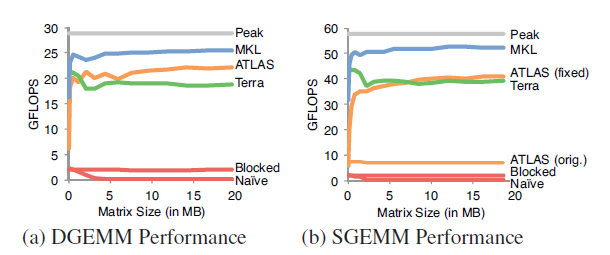
\includegraphics[scale=0.5]{terra3.png}
  \end{center}
\end{frame}

\begin{frame}
	\frametitle{Summary}
  \begin{itemize}
  \item Two-Languages design: Lua + Terra.\pause
  \item Shared lexical scoping.\pause
  \item Seperate Evaluationn: Lua(LuaJIT), Terra(LLVM JIT).\pause
  \item Type Reflection.
  \end{itemize}
\end{frame}

\begin{frame}
	\frametitle{Advantages}
  \begin{itemize}
  \item No need to write C, but the performance is still good.\pause
  \item Generating code dynamically allows us to use runtime information from LuaJIT.\pause
  \item Easy to re-use C/C++ libraries in Lua.\pause
  \end{itemize}
\end{frame}

\begin{frame}
	\frametitle{Shortages}
  \begin{itemize}
  \item Lua is not statically typed.
  \end{itemize}
\end{frame}

\begin{frame}
	\frametitle{Reference}
  \begin{itemize}
  \item Zachary DeVito, James Hegarty, Alex Aiken, Pat Hanrahan, and Jan Vitek. 2013. Terra: A multi-stage language for high-performance computing. In Proceedings of the 34th ACM SIGPLAN Conference on Programming Language Design and Implementation (PLDI’13). ACM, New York, 105–116. DOI:\url{https://doi.org/10.1145/2491956.2462166}
  \item Terra: A low-level counterpart to Lua. \url{https://terralang.org/}
  \end{itemize}
\end{frame}

\end{document}

